\begin{document}
\documentclass[french, a4, 10pt]{article} % si la table des matiï¿œes est petite
\usepackage[utf8]{inputenc}
\usepackage[francais]{babel}
% Modification des marges ------------------------------
\oddsidemargin -4mm 	% Marge de gauche -4mm
\textwidth 17cm 	% Largeur de gauche = 17cm
\textheight 22cm 	% Hauteur du texte = 22cm
\parindent 0cm		% Pas d'indentation de paragraphe
% -----------------------------------------------------
\usepackage[T1]{fontenc}
\usepackage{graphicx,color, caption2}
\usepackage{epsfig}
\usepackage{fancyhdr}
%\usepackage{fancyvrb}
\usepackage{textcomp}
\pagestyle{fancy}
\usepackage{listings}		% pour incorporer des sources
\usepackage[francais]{layout}	% pour obtenir le layout
\usepackage{fullpage}		% pour obtenir le layout
\usepackage{makeidx}		% pour créer une table d'index
\begin{document}
% Titres sur  chaque page -----------------------------
\lhead{ } % Haut gauche
%\chead{Haut centre}
\rhead{Ecrire un rapport en latex}
\lfoot{\copyright{Jaumain Jean-Claude}}
\cfoot{ } % Bas centre - obligatoire !
\rfoot{\thepage} % Bas droite
\renewcommand{\headrulewidth}{0.4pt} 
\renewcommand{\footrulewidth}{0.4pt} 
% Numérotation et table des matières -----------------
\setcounter{tocdepth}{1}    % fixe la profondeur de la table des matières
\setcounter{secnumdepth}{5} % fixe la profondeur de la numérotation des sections et paragraph
% Page de garde --------------------------------------
\title{\emph{\textbf{Écrire un rapport en Latex}}}
\author{Jaumain J-C}
\date{15 septembre 2010}
\maketitle
\tableofcontents
% Inclusion des textes
\section{Introduction}
L'objectif de ce travail est de fournir une base pour celui qui doit écrire un rapport pour mon cours. Il commence par une suite d'exemples suffisante pour pouvoir établir un premier rapport correct. Ensuite, une série d'autres exemples montre comment améliorer sa présentation pour l'étudiant qui le souhaite. Ce rapport, comme celui de l'étudiant doit comporter un titre, une table des matières, un résumé de l'objectif poursuivi, le texte découpé en chapitres, une conclusion, les références et le contenu du répertoire associé.  
%-----------------------------------------------------------------------------------
\section {Une première approche très simple}
Vous découpez votre travail en chapitre (section), en sous-chapitre (subsection) et en sous-sous-chapitre (subsubsection)
\subsection {Un chapitre simple}
Il suffit de taper le texte au kilomètre. \emph{Il est possible d'insister} sur un passage.
\subsection {Vérification de l'orthographe}
Vous appelez la commande :
\lstset{frame=trBL}
\begin{lstlisting}
aspell -t - -encoding='iso8859-15' -c VotreFichier.tex
\end{lstlisting}
\subsection {Une énumération}
Si vous devez utiliser des puces :
\begin{itemize}
\item point 1
\item point 2
\end{itemize}
Si vous devez énumérer :
\begin{enumerate}
\item point 1
\item point 2
\end{enumerate}
Vous pouvez mélanger à autant de niveaux que vous le souhaitez.
\subsection{Un tableau}
\begin{tabular}{|l|l||c||r|} %left ou r ou c ou p[dimension]
\hline
Jour & Heures & Local & Cours \\
\hline
Mardi    &  3..4  & 503 & Système\\
Mardi    &  5..8  & 503 & Sécurité\\
\hline
Mercredi  &  1..2  &  201 & Assembleur\\
Mercredi  &  3..4  &  003 & Labo assembleur\\
\hline
\end{tabular}
\subsection {Intégrer une source}
Pour énumérer une source, vous pouvez préciser ce que vous souhaitez avec lstset. 
\lstset{language={},frame=trBL}
\begin{lstlisting}
MOV EAX,10 ; place 10 dans le registre EAX
ADD EAX,20 ; ajoute 20 au contenu de EAX
\end{lstlisting}
\subsection {Intégrer un graphique}
Vous pouvez intégrer un graphique mais il faut qu'il soit en format eps.\\
Vous pouvez dessiner avec l'outil oodraw qui permet d'exporter votre dessin dans ce format eps.\\
Vous pouvez transformer un jpeg en eps avec l'outil sam2p ou convert qui se trouve dans le package ImageMagick\\
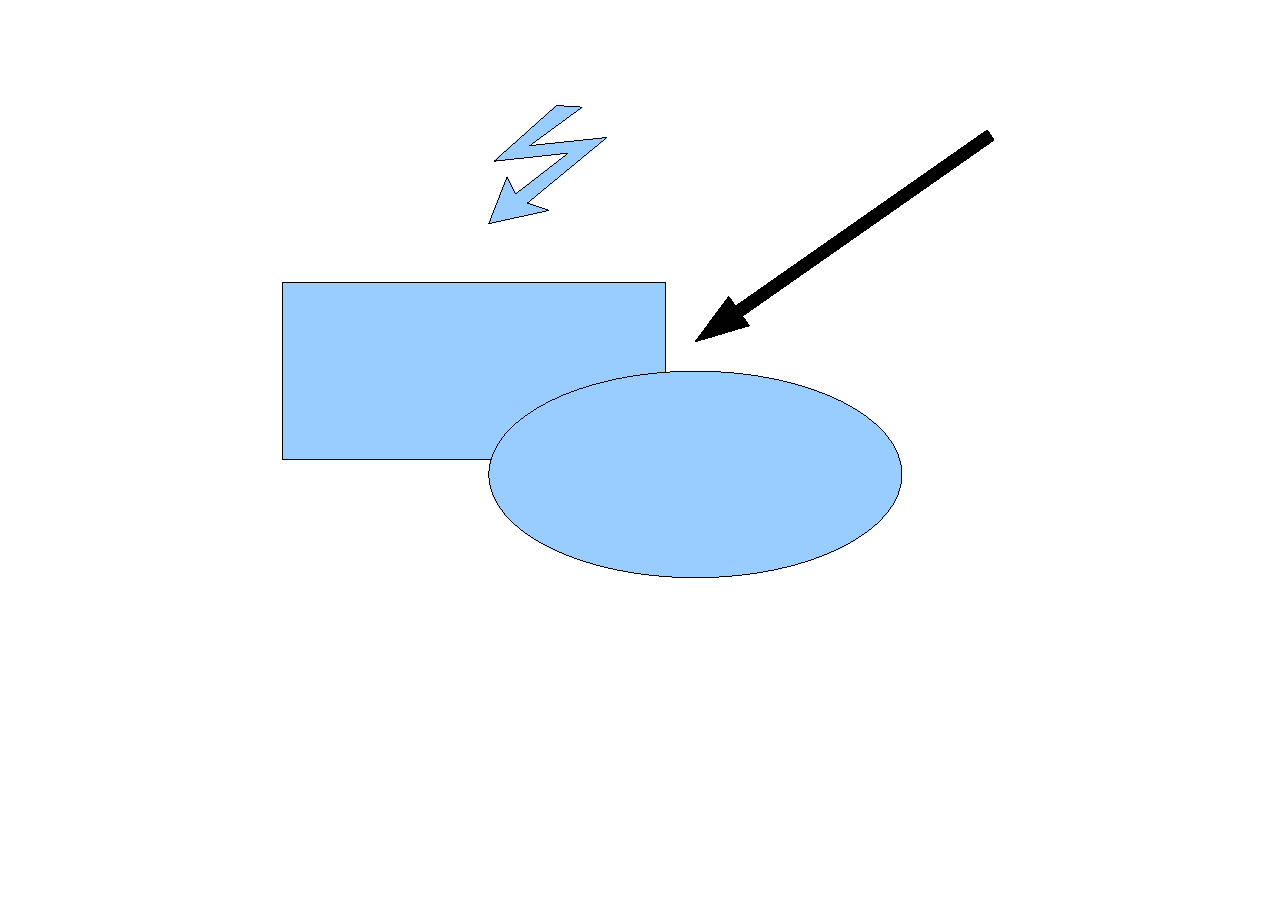
\includegraphics[width=8cm]{Dessin.eps}
\subsection {Mode mathématique}
C'est un des points forts de latex qui permet d'écrire des formules mais aussi des caractères spéciaux tels que :
$2^{32} \approx 10^{9}$ car $\log{_{10}}{2} \approx 0.3$ et $32*0.3 \approx 9$.
\subsection {Quelques trucs faciles}
\begin{itemize}
\item \verb+\\+ permet de passer à la ligne suivante.
\item \verb+\\[2cm]+ permet de passer à la ligne suivante + une tabulation verticale de 2cm. Sont autorisés mm, cm et pts.
\item \verb+\newpage+ permet de forcer un passage à la page suivante.
\end{itemize}
\subsection {Compiler le texte}
Un script permet d'automatiser cette compilation:
\begin{lstlisting}
#! /bin/sh
FN=Mrapport # Le nom du document.
latex $FN.tex
latex $FN.tex # 2 passages pour la TOC
rm $FN.aux $FN.log $FN.out
dvips $FN.dvi -o $FN.ps
rm $FN.dvi
gv $FN.ps # pour visualiser et imprimer
\end{lstlisting}
%-----------------------------------------------------------------------------------
\section{Conclusions}
Ce travail montre, qu'en quelques minutes, on peut déjà fournir un travail présenté de façon professionnelle, lisible par tous et dans un format standard.
Pour ne pas avoir de soucis, les commandes à utiliser pour obtenir un document postcript sont latex et dvips, il ne faut jamais utiliser pdflatex. 

Ce document peut être encore complété avec d'autres exemples qui seraient utiles. Ces nouveaux exemples pourraient être intégrés dans le premier ou un deuxième chapitre. Ceci, sans oublier qu'il s'agit d'un document utile pour commencer très rapidement à écrire en latex et non un mode d'emploi complet de latex qui serait obligatoirement très volumineux.
%-----------------------------------------------------------------------------------
\section{Références}
\begin{itemize}
\item http://www.grappa.univ-lille3.fr/FAQ-LaTeX/ 
\item http://tex.loria.fr/
\item http://tex.loria.fr/english/packages.html
\end{itemize}
%-----------------------------------------------------------------------------------
\section{Annexes }
Vous trouvez dans le casier, un répertoire LATEX contenant :
\begin{itemize}
\item Mrapport.tex : le document latex maître
\item LatexSimple.tex : ce document latex
\item dessin.odg et dessin.eps : le dessin intégré dans le texte
\item go : un script qui permet de compiler rapport.tex, sans argument.
\end{itemize}
%-----------------------------------------------------------------------------------


\section{Mathématiques}
% use package amsmath, amsfont, amssymb peuvent être utiles.
\index{équation}
Quelques exemples des possibilités mathématiques :

La fonction $e^x$ est strictement croissante sur $R$ et $\forall x \in R$.

\begin{equation}
\frac{\partial}{\partial y}\int_E f(x,y)\,dx = \int_E \frac{\partial f(x,y)}{\partial y}\,dx
\end{equation}

$$\lim_{x \to +\infty} \frac{\ln x}{x} = 0$$

$$ 10 \textrm{ dixièmes} = 1 $$

\begin{equation}
\sum_{k=1}^n k = \frac{n(n+1)}{2}
\end{equation}

\begin{equation}
\int_0^{+\infty} x^n e^{-x}\,dx = n!
\end{equation}

$$\left \{\begin{array}{c}x+y=1\\x-y=1\end{array}\right.$$

\begin{equation}
\left( \begin{array}{cc} a & b \\ c & d \end{array} \right) \cdot
\left( \begin{array}{cc} 0 & 1 \\ 0 & 0 \end{array} \right) =
\left( \begin{array}{cc} 0 & a \\ 0 & c \end{array} \right)
\end{equation}

$$\widehat{ab} + \widehat{bc} + \widehat{cb} = 180$$

$$\overrightarrow{ab} + \overrightarrow{ac} = \overrightarrow{ad}$$
 % pas de saut de page
\section{Intégrer une source}
\subsection{Configuration de lstlisting}
% Le manuel se trouve dans le howto ou dans CTAN sous le nom de listings.pdf
La commande lstset permet de fixer la présentation des sources. Il n'est pas conseillé d'utiliser utf8 pour les sources si le document n'est pas en utf8.
\lstset{language={},%C,Assembleur, TeX, tcl, basic, cobol, fortran, logo, make, pascal, perl, prolog, {}
	literate={â}{{\^a}}1 {ê}{{\^e}}1 {î}{{\^i}}1 {ô}{{\^o}}1 {û}{{\^u}}1
		 {ä}{{\"a}}1 {ë}{{\"e}}1 {ï}{{\"i}}1 {ö}{{\"o}}1 {ü}{{\"u}}1
		 {à}{{\`a}}1 {é}{{\'e}}1 {è}{{\`e}}1 {ù}{{\`u}}1 
		 {Â}{{\^A}}1 {Ê}{{\^E}}1 {Î}{{\^I}}1 {Ô}{{\^O}}1 {Û}{{\^U}}1
		 {Ä}{{\"A}}1 {Ë}{{\"E}}1 {Ï}{{\"I}}1 {Ö}{{\"O}}1 {Ü}{{\"U}}1
		 {À}{{\`A}}1 {É}{{\'E}}1 {È}{{\`E}}1 {Ù}{{\`U}}1,
	commentstyle=\scriptsize\ttfamily\slshape, % style des commentaires
	basicstyle=\scriptsize\ttfamily, % style par défaut
	keywordstyle=\scriptsize\rmfamily\bfseries,% style des mots-clés
	backgroundcolor=\color[rgb]{.95,.95,.95}, % couleur de fond : gris clair
	framerule=0.5pt,% Taille des bords
	frame=trbl,% Style du cadre
	frameround=tttt, % Bords arrondis 
	tabsize=3, % Taille des tabulations
%	extendedchars=\true, % Incompatible avec utf8 et literate
	inputencoding=utf8,
	showspaces=false, % Ne montre pas les espaces 
	showstringspaces=false, % Ne montre pas les espaces entre ''
	xrightmargin=-1cm, % Retrait gauche 
	xleftmargin=-1cm, % Retrait droit
	escapechar=@}  % Caractère d'échappement, permet des commandes latex dans la source
% -----------------------------------------------------
\subsection{Intégrer une source dans le texte}
\begin{lstlisting}
/*---------------------------------------------------------------------------------------
NOM      : Exemple.c
CLASSE   : Applications - Latex - Illustration
OBJET    : Sert d'exemple pour inclure une source en latex
         : Dans ce ces, ce programme affiche Hello
HOWTO    : gcc Exemple.c -o Exemple; ./Exemple
AUTEUR   : J.C. Jaumain, le 3/11/2010
BUGS     :  /
REMARQUE : Impose lstset {escapechar=@\symbol{64}@} pour l'interprétation des balises latex
----------------------------------------------------------------------------------------*/
main() {
	int i;  // Pour récupérer le nombre de caractères écrits
	tab[10] Buffer='Hello'; // Le buffer
	i=write(1,Buffer,5); // La @$\frac{1}{2}$@ du buffer
	exit(0);
}
\end{lstlisting}

L'intérêt de cette technique est de figer le source et d'avoir un document autonome

\subsection{Intégrer une source d'un fichier}

\lstinputlisting{Exemple.c}

L'intérêt de cette technique est d'avoir un source toujours "à jour".




\section{Tables}

\subsection{Table des matières}

La commande tableofcontents permet d'insérer une table des matières à cet endroit. Il faut compiler deux fois le document pour que la table des matières soit correcte. Au premier passage, le compilateur crée un fichier.toc qui servira lors de la deuxième compilation.

La variable tocdepth permet de fixer les niveaux repris dans la table des matières.

\subsection{Table des index}
\index{makeidx}
\index{makeindex} 
\index{printindex} 
\index{index}
En utilisant le package "makeidx", la commande makeindex permet de créer une table des index. La commande printindex permet d'insérer une table des index à cet endroit. Il faut compiler deux fois le document pour que la table des index soit correcte. Au premier passage, le compilateur crée des fichiers d'index qui serviront lors de la deuxième compilation. La commande makeindex citée ci-dessus est à exécuter entre les deux compilation.\\
Pour qu'un terme soit repris dans la table des index, il faut utiliser la commande 
\verb+\index{Nom de l'item}+.


\section{Mise en page}

\subsection{Marges...}

Une série de variables définissent la mise en page. En utilisant les packages [francais]{layout} et {fullpage}, on peut utiliser la commande layout qui permet d'ajouter une page qui dessine la présentation d'une page et les noms des variables assignées.

\layout

On peut ensuite modifier ce que l'on souhaite :
\begin{verbatim}
% Modification des marges ------------------------------
\oddsidemargin -4mm 	% Marge de gauche -4mm
\textwidth 17cm 	% Largeur de gauche = 17cm
\textheight 22cm 	% Hauteur du texte = 22cm
\parindent 0cm		% Pas d'indentation de paragraphe
% -----------------------------------------------------
\end{verbatim}

\subsection{Niveaux}

Vous avez droit à la structure

\begin{list}{$\bullet$}{}
\item part avec saut de page
\item chapter : niveau 0
\item section : niveau 1
\item subsection : niveau 2
\item subsubsection : niveau 3
\item paragraph : niveau 4
\item subparagraph : niveau 5
\end{list}

La variable secnumdepth permet de limiter la numérotation des niveaux. Par exemple, la valeur 5 permet d'avoir une numérotation du style 1.2.3.2.1.2 pour le subparagraph\footnote{De la même façon, on peut limiter le nombre de niveaux affichés dans une table des matières avec la variable tocdepth }. 
(Il est toujours possible d'insérer une note de bas de page avec \verb+\footnote+)

\subsection{Cadres}

Il est possible d'encadrer un mot avec \fbox{box}

%\shabox{On peut aussi encadrer tout un paragraphe avec l'environnement shabox à condition de déclarer le package shadow avant le début du document}.

\section{Couleurs à volonté}

\index{RGB}

\noindent 
Le package couleur permet de définir des couleurs en donnant les quantités de rouge, de vert
et de bleu (RGB). Ces quantités varient de 0.0 à 1.0.

\begin{lstlisting}
\definecolor{rouge}{rgb}{1.0,0.0,0.0}
\definecolor{noir}{rgb}{0.0,0.0,0.0}
\end{lstlisting}

permettent d'utiliser ces deux nouvelles couleurs :

\begin{lstlisting}
\noindent\color{rouge}Essai de couleur\\
\color{noir}Essai de couleur numéro 2
\end{lstlisting}

ce qui donne :

\definecolor{rouge}{rgb}{1.0,0.0,0.0}
\definecolor{noir}{rgb}{0.0,0.0,0.0}
\noindent\color{rouge}Essai de couleur\\
\color{noir}Essai de couleur numéro 2\\

\section{Programmation}

% \subsection{Variables}   REPRENDRE LES SLIDES
% 
% Deux sortes de variables : les entiers et les dimensions. Les dimensions sont toujours accompagnées d'une unité. (mm, cm, pt,...)
% 
% \subsubsection{variables}
% \begin{itemize}
% \item Création : 
% \item Assignation :
% \item Incrémentation :
% \item Tests :
% \end{itemize}
% 
% \subsubsection{variables prédéfinies}
% \begin{itemize}
% \item 
% \item 
% \item 
% \item 
% \item 
% \item 
% \item 
% \item 
% \item 
% \item 
% \item 
% \end{itemize}
% 
% \subsubsection{dimensions}
% \begin{itemize}
% \item Création : 
% \item Assignation :
% \item Incrémentation :
% \item Tests :
% \end{itemize}
% 
% \subsubsection{dimensions prédéfinies}
% \begin{itemize}
% \item 
% \item 
% \item 
% \item 
% \item 
% \item 
% \item 
% \item 
% \item 
% \item 
% \item 
% \end{itemize}
% 
% 
% \section{contrôles}
% 
\section{commandes}

\begin{verbatim}
\newcommand{\NomCmd}[argc][def1]
{ Commandes où les arguments s'appellent #1 #2...
}
ou \renewcommand...
\end{verbatim}
où
\begin{itemize}
\item NomCmd est le nom donné à la commande 
\item argc est le nombre d'argument, 0 par défaut
\item def1 est une valeur par défaut pour le premier argument.
\item newcommand pour définir une nouvelle commande dont le nom n'existe pas 
\item renewcommand pour redéfinir une commande dont le nom existe déjà 
\end{itemize}

\subsection{Exemples:}

\newcommand{\EtatCivil}[3]{\textbf{#1} #2 #3}
\EtatCivil{M.}{Albert}{Einstein}\\
\renewcommand{\EtatCivil}[3][M.]{\textbf{#1} #2 #3}
\EtatCivil{Albert}{Einstein}\\
\EtatCivil[Mme]{Julio}{Curie}\\

% \section{environnement}    NE FONCTIONNE PAS !!!!
% 
% \begin{verbatim}
% \newenvironment{NomEnv}[argc][def1]
% {sequenceDebut}{SectionFin} où les arguments s'appellent #1 #2...
% \end{verbatim}
% où
% \begin{itemize}
% \item NomEnv est le nom donné à l'environnement 
% \item argc est le nombre d'argument, 0 par défaut
% \item def1, optionnel, est une valeur par défaut pour le premier argument.
% \item newenvironment pour définir un nouvel environnement dont le nom n'existe pas 
% \end{itemize}
% 
% \subsection{Exemples:}
% 
% \newenvironment{MonTitre}[1]{\
% begin{center}\textbf{#1}\\}{\end{center}}
% 
% \begin{MonTitre}{Première ligne}
% Ligne deuxième
% \end{MonTitre}



%\include{Latex}
%\include{Latex}
\printindex			% Impression de la table des index
\end{document}











% Titres sur  chaque page -----------------------------
\lhead{ } % Haut gauche
%\chead{Haut centre}
\rhead{Ecrire un rapport en latex}
\lfoot{\copyright{Jaumain Jean-Claude}}
\cfoot{ } % Bas centre - obligatoire !
\rfoot{\thepage} % Bas droite
% Numérotation et table des matières -----------------
\setcounter{tocdepth}{1}    % fixe la profondeur de la table des matières
\setcounter{secnumdepth}{3} % fixe la profondeur de la numérotation des sections et paragraph
% Page de garde ---------------------------
\title{\emph{\textbf{Raconter en Latex}}}
\author{M Bastreghi}
\date{22 septembre 201}
\maketitle
\tableofcontents
% Inclusion des textes
\printindex			% Impression de la table des index
\end{document}
